\documentclass[english,11pt]{beamer}

\DeclareMathOperator{\Cov}{Cov}
\DeclareMathOperator{\Var}{Var}
\DeclareMathOperator{\E}{\mathbb{E}}
\DeclareMathOperator{\Proba}{\mathbb{P}}

\newcommand{\Covb}[2]{\ensuremath{\Cov\!\left[#1,#2\right]}}
\newcommand{\Eb}[1]{\ensuremath{\E\!\left[#1\right]}}
\newcommand{\Pb}[1]{\ensuremath{\Proba\!\left[#1\right]}}
\newcommand{\Varb}[1]{\ensuremath{\Var\!\left[#1\right]}}

% norm
\newcommand{\norm}[1]{\| #1 \|}

\newcommand{\indep}{\rotatebox[origin=c]{90}{$\models$}}





\usepackage{mathptmx,amsmath,amssymb,graphicx,bibentry,bbm,babel,ragged2e}

\makeatletter

\newcommand{\noun}[1]{\textsc{#1}}
\newcommand{\jitem}[1]{\item \begin{justify} #1 \end{justify} \vfill{}}
\newcommand{\sframe}[2]{\frame{\frametitle{#1} #2}}

\newenvironment{centercolumns}{\begin{columns}[c]}{\end{columns}}
%\newenvironment{jitem}{\begin{justify}\begin{itemize}}{\end{itemize}\end{justify}}

\usetheme{Warsaw}
\setbeamertemplate{footline}[text line]{}
\setbeamertemplate{headline}{}
\setbeamercolor{structure}{fg=purple!50!blue, bg=purple!50!blue}

\setbeamersize{text margin left=15pt,text margin right=15pt}

\setbeamercovered{transparent}


\@ifundefined{showcaptionsetup}{}{%
 \PassOptionsToPackage{caption=false}{subfig}}
\usepackage{subfig}

\usepackage[utf8]{inputenc}
\usepackage[T1]{fontenc}

\usepackage{multirow}


\makeatother




\begin{document}

\title{A meta-analysis of models for interactions between transportation networks and territories}
\author{J.~Raimbault$^{1,2,3\ast}$\\
\texttt{j.raimbault@ucl.ac.uk}
}


\institute{$^{1}$CASA, UCL\\
$^{2}$UPS CNRS 3611 Complex Systems Institute Paris\\
$^{3}$UMR CNRS 8504 G{\'e}ographie-cit{\'e}s
}


\date{ECTQG 2019\\
Co-evolution of cities and networks\\
September 8th 2019
}

\frame{\maketitle}


% 
%\textbf{Keywords: }\textit{Network-territories interaction models; Systematic review; Meta-analysis}



\sframe{Interactions between networks and territories}{

% The dynamics of territorial systems have extensively been studied in their interaction with transportation networks which are assumed to play a significant role in their trajectories.

% CN quali slide


\justify

\begin{center}
\includegraphics[width=0.45\linewidth]{figures/accessp_withbridge_prd_EN.png}
\hspace{0.1cm}
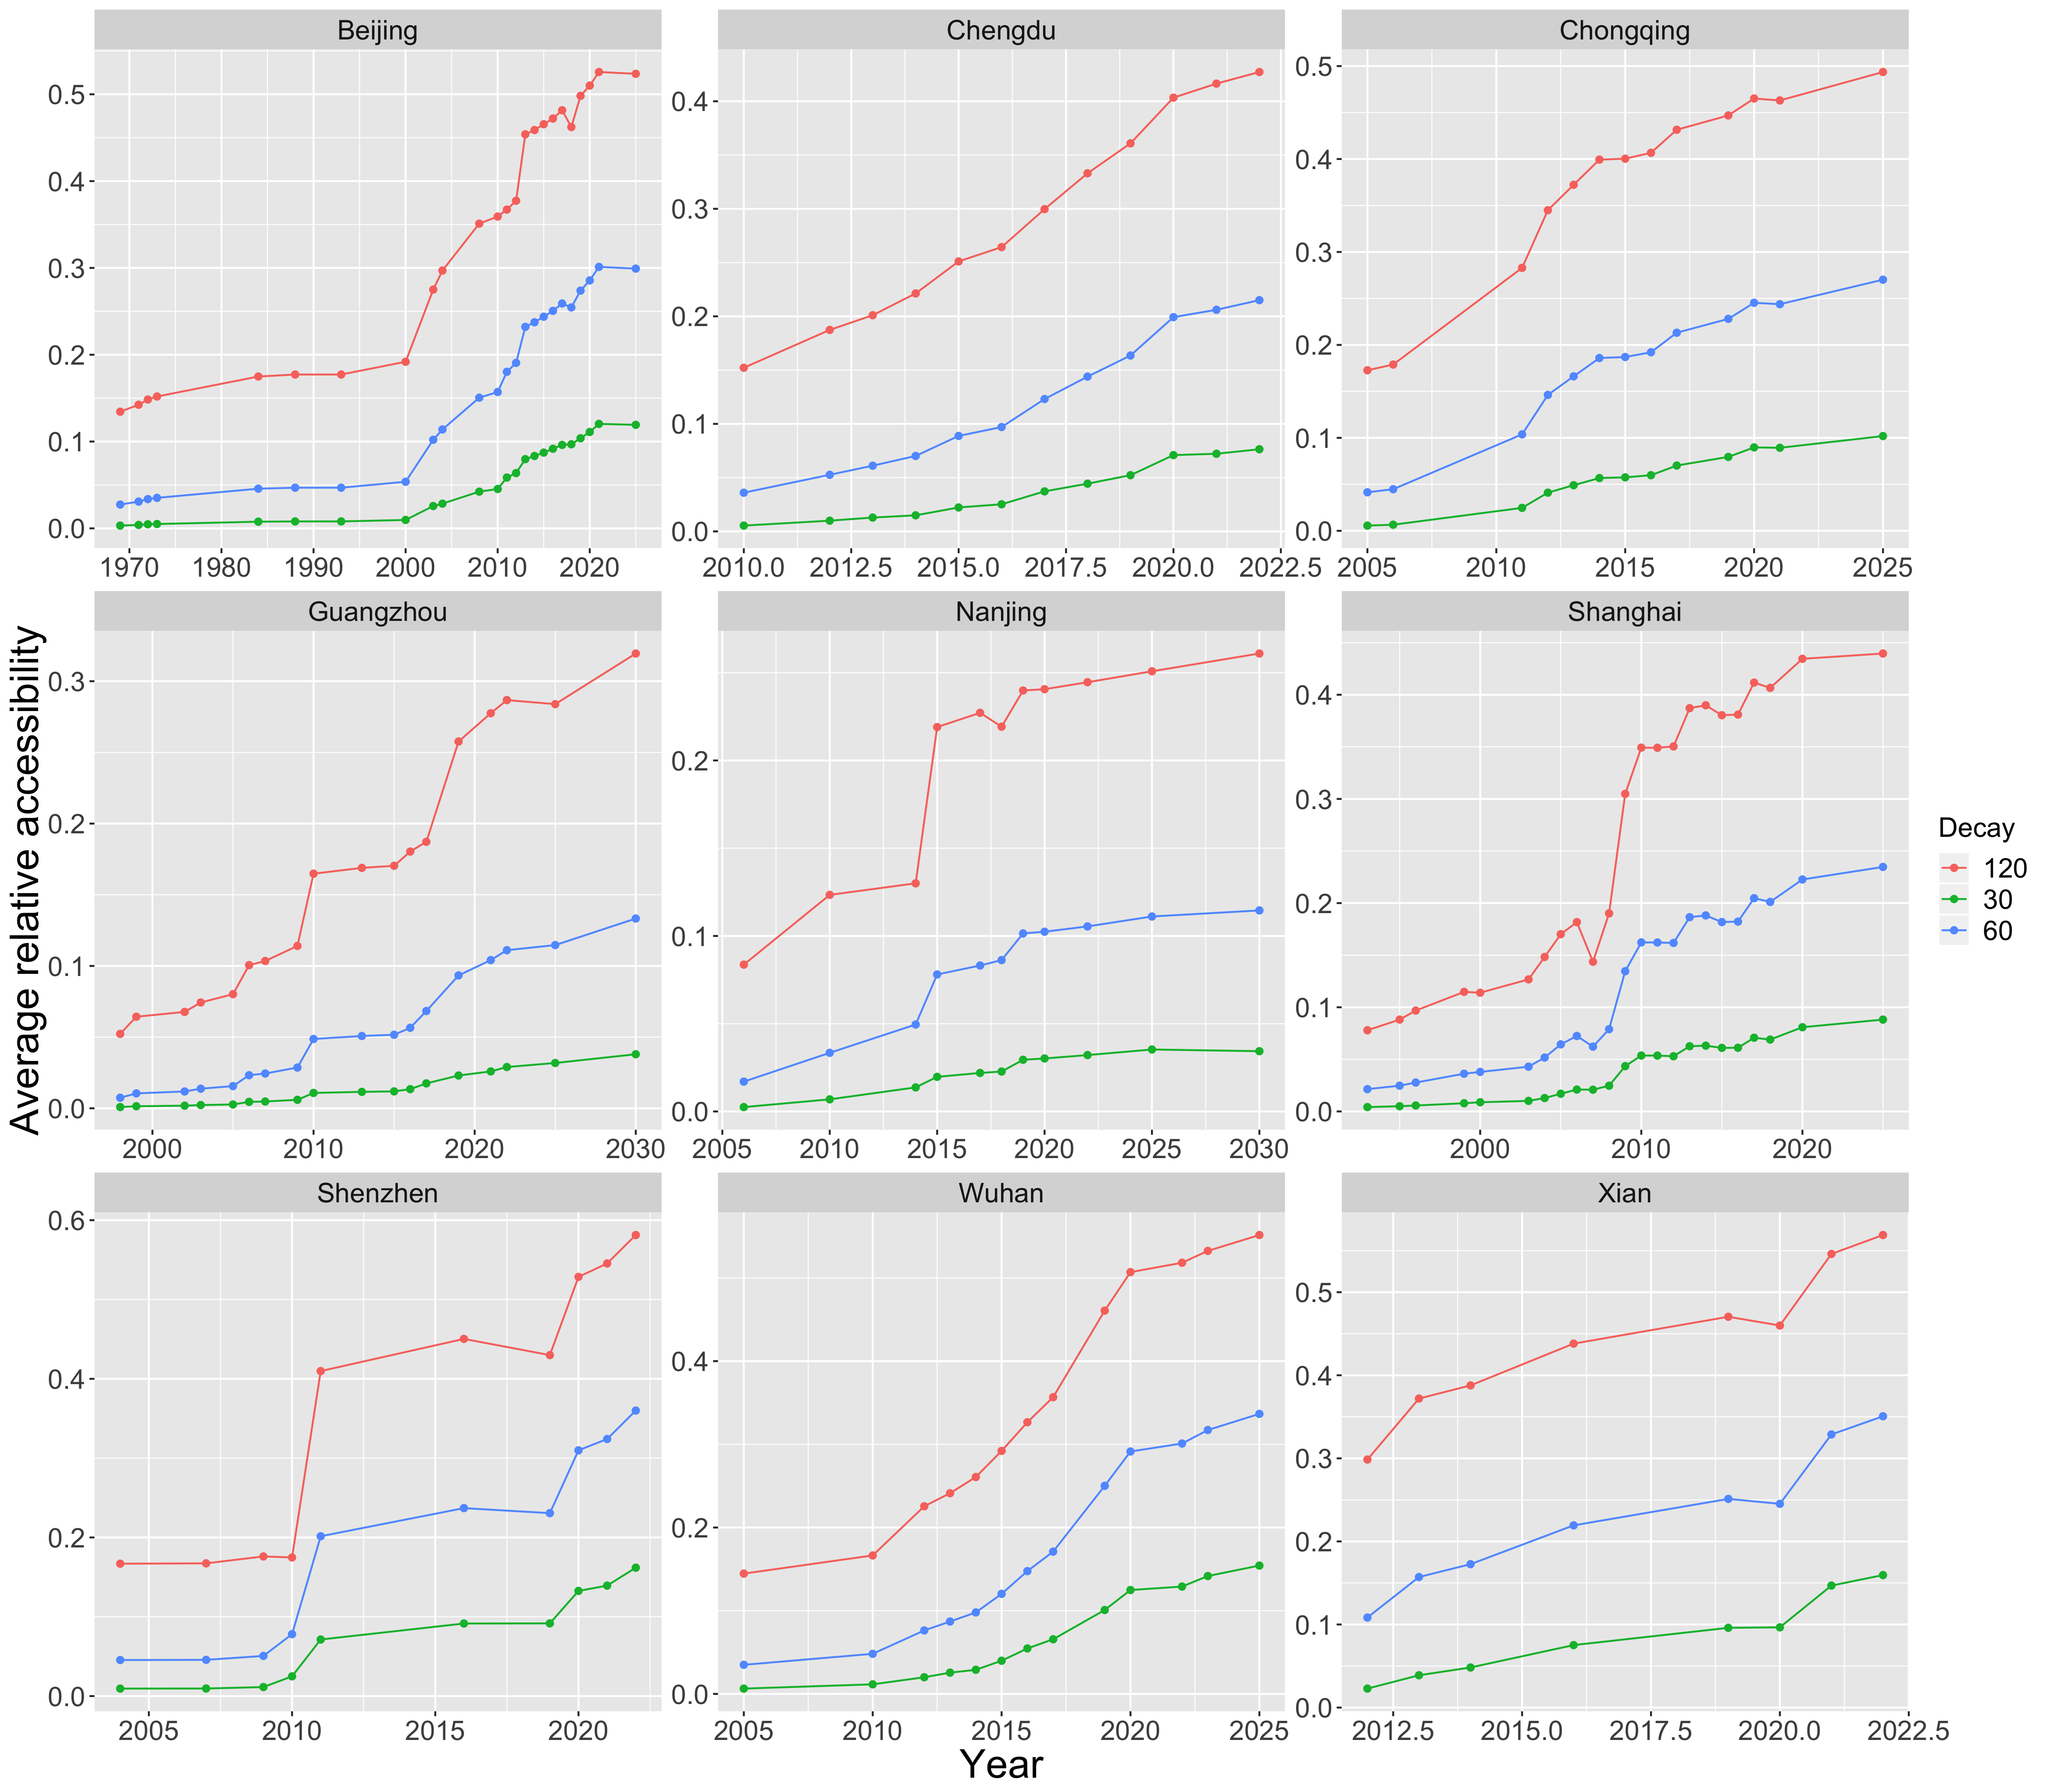
\includegraphics[width=0.52\linewidth]{figures/avgaccess_facet.png}

\end{center}

\medskip

%\vspace{-0.5cm}

%\begin{justify}
\textit{Accessibility as part of complex processes of co-evolution between transportation networks and territories.}

%\end{justify}

\nocite{raimbault:halshs-02265423}

\medskip

\tiny

Raimbault, J. (2019). Evolving accessibility landscapes: mutations of transportation networks in China. In Aveline-Dubach, N., ed. \textit{Pathways of sustainable urban development across China - the cases of Hangzhou, Datong and Zhuhai}, pp 89-108. Imago. ISBN:978-88-94384-71-0

}



\sframe{}{

% processes from the lit review / chap 1 ?



}


\sframe{Diverse modeling approaches}{

% Therefore, several modeling approaches focusing on the interactions between transportation networks and territories have been introduced by various disciplines, including for example land-use transport interaction models from planning and transportation science, spatial interaction models or co-evolution models from geography, network growth models from physics.

% -> cit nw analysis ectqg 2017

\textit{Complementary modeling approaches}

\medskip

\begin{center}
	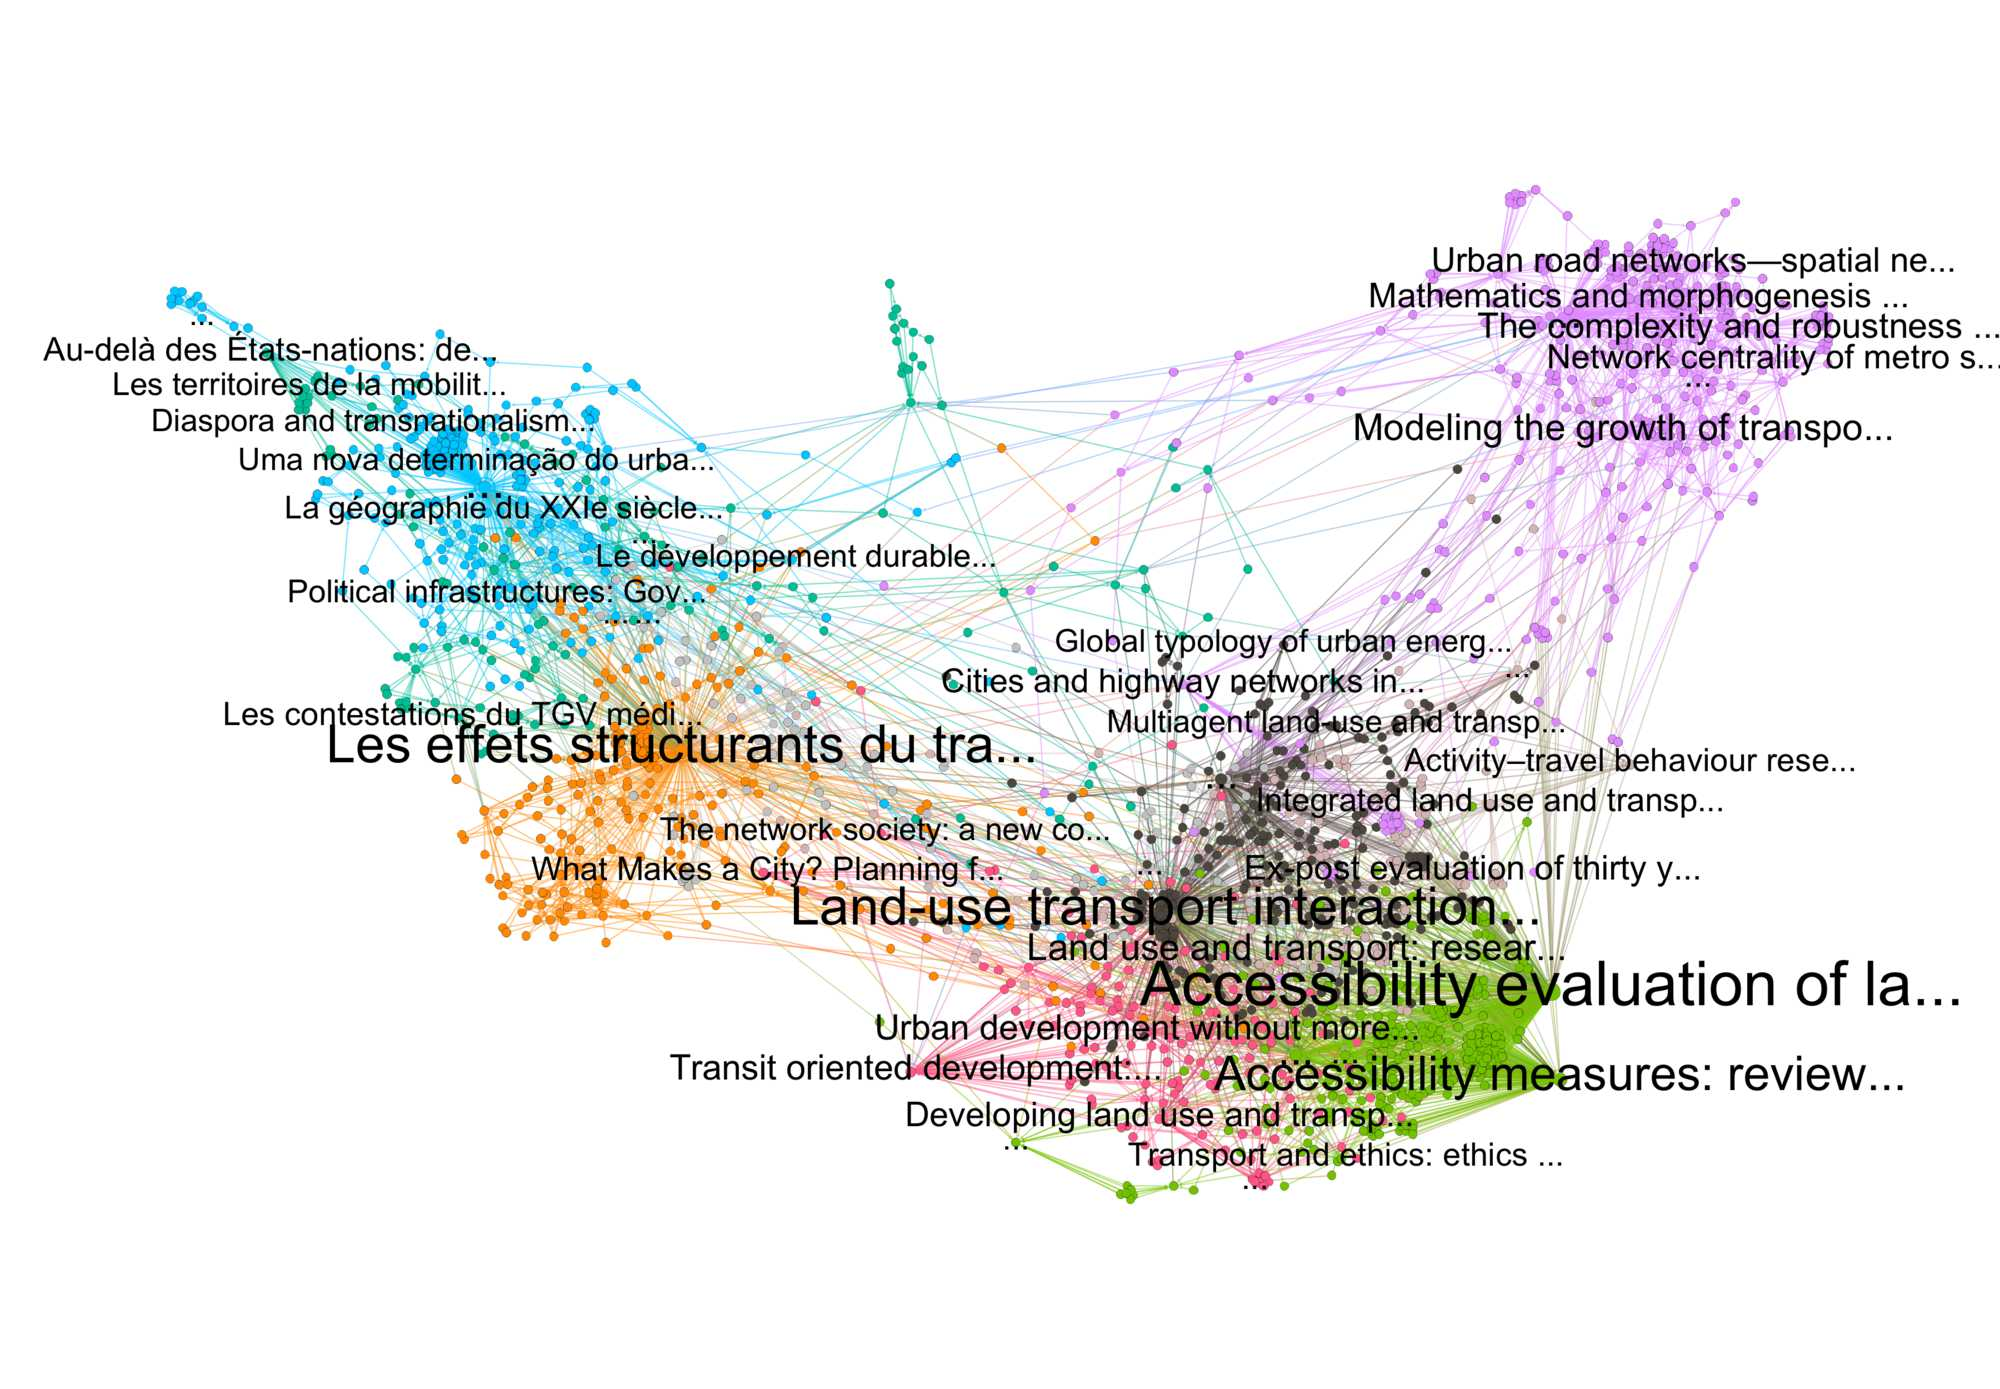
\includegraphics[width=0.9\textwidth,trim={0 2cm 0 2cm},clip]{figures/2-2-2-fig-quantepistemo-citnw.jpg}	
\end{center}

\medskip

\tiny

\vspace{-1cm}

Raimbault, J. (2019). Exploration of an interdisciplinary scientific landscape. Scientometrics, 119(2), 617-641.

\nocite{raimbault2019exploration}

}


\sframe{Towards a modelography}{

%  This contribution introduces a systematic review and meta-analysis to understand the nature and properties of these models in relation to their disciplinary context.

% research question



}


\sframe{Corpus construction method}{

%We construct a corpus of models through a systematic review. The raw corpus after initial keyword requests is composed by around 3800 papers, which were screened for inclusion first on their titles (297 papers kept), then on their full-text content resulting in a study corpus of 145 papers.


}


\sframe{Extracted characteristics}{

%For each model, properties are extracted including the type of coupling (weak or strong and the direction) between network and territory, spatial and temporal scales, the methodology used, and the discipline, in order to proceed to a meta-analysis of these.



}


\sframe{}{

%Exploratory analysis confirms the diversity of approaches existing, 


}


\sframe{}{

%whereas statistical analysis links type of models and disciplines with properties, showing for example the strong influence of the type of coupling with time scale, or of the discipline on the spatial scale.


}


\sframe{}{

%We finally use random forest regression to compare the relative importance of variables to explain model type, and show that among different way to define disciplinary belonging, position in the citation network has the largest influence.


}


\sframe{}{

% synthesis : modeled processes ?
% + content of thesis models ?

}





\sframe{Discussion}{

 % This work thus provide a systematic and broad overview on the diversity of approaches to model interaction between networks and territories, and foster the possibilities of a reflexive positioning in the context of building new models.


}



\sframe{Conclusion}{

 % need of reflexivity : cite complexities ?

}





\sframe{Reserve slides}{

\centering

\Large

\textbf{Reserve Slides}

}


% - full stat models
% - pareto optim for model selection




%%%%%%%%%%%%%%%%%%%%%
\begin{frame}[allowframebreaks]
\frametitle{References}
\bibliographystyle{apalike}
\bibliography{biblio}
\end{frame}
%%%%%%%%%%%%%%%%%%%%%%%%%%%%







\end{document}




